\section{Конструкторский раздел}

\subsection{Проектирование базы данных}

На рисунке \ref{fig:erd} представлена схема проектируемой базы данных.

\begin{figure}[H]
	\centering
	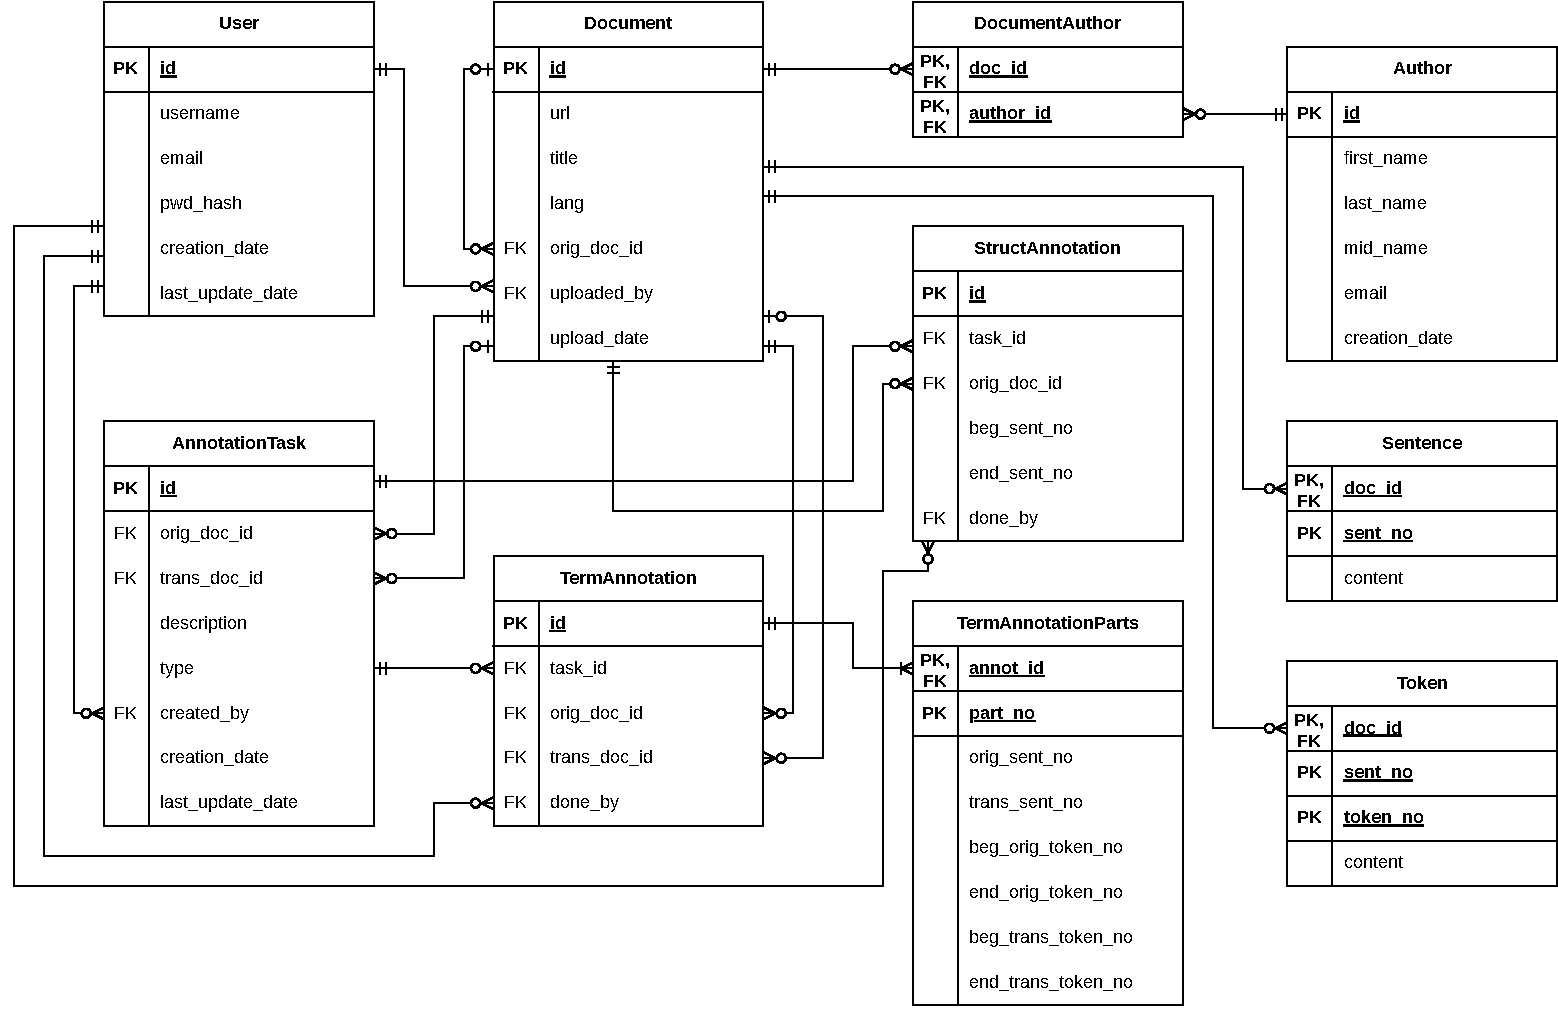
\includegraphics[width=\textwidth]{diag/crow-foot-erd.pdf}
	% 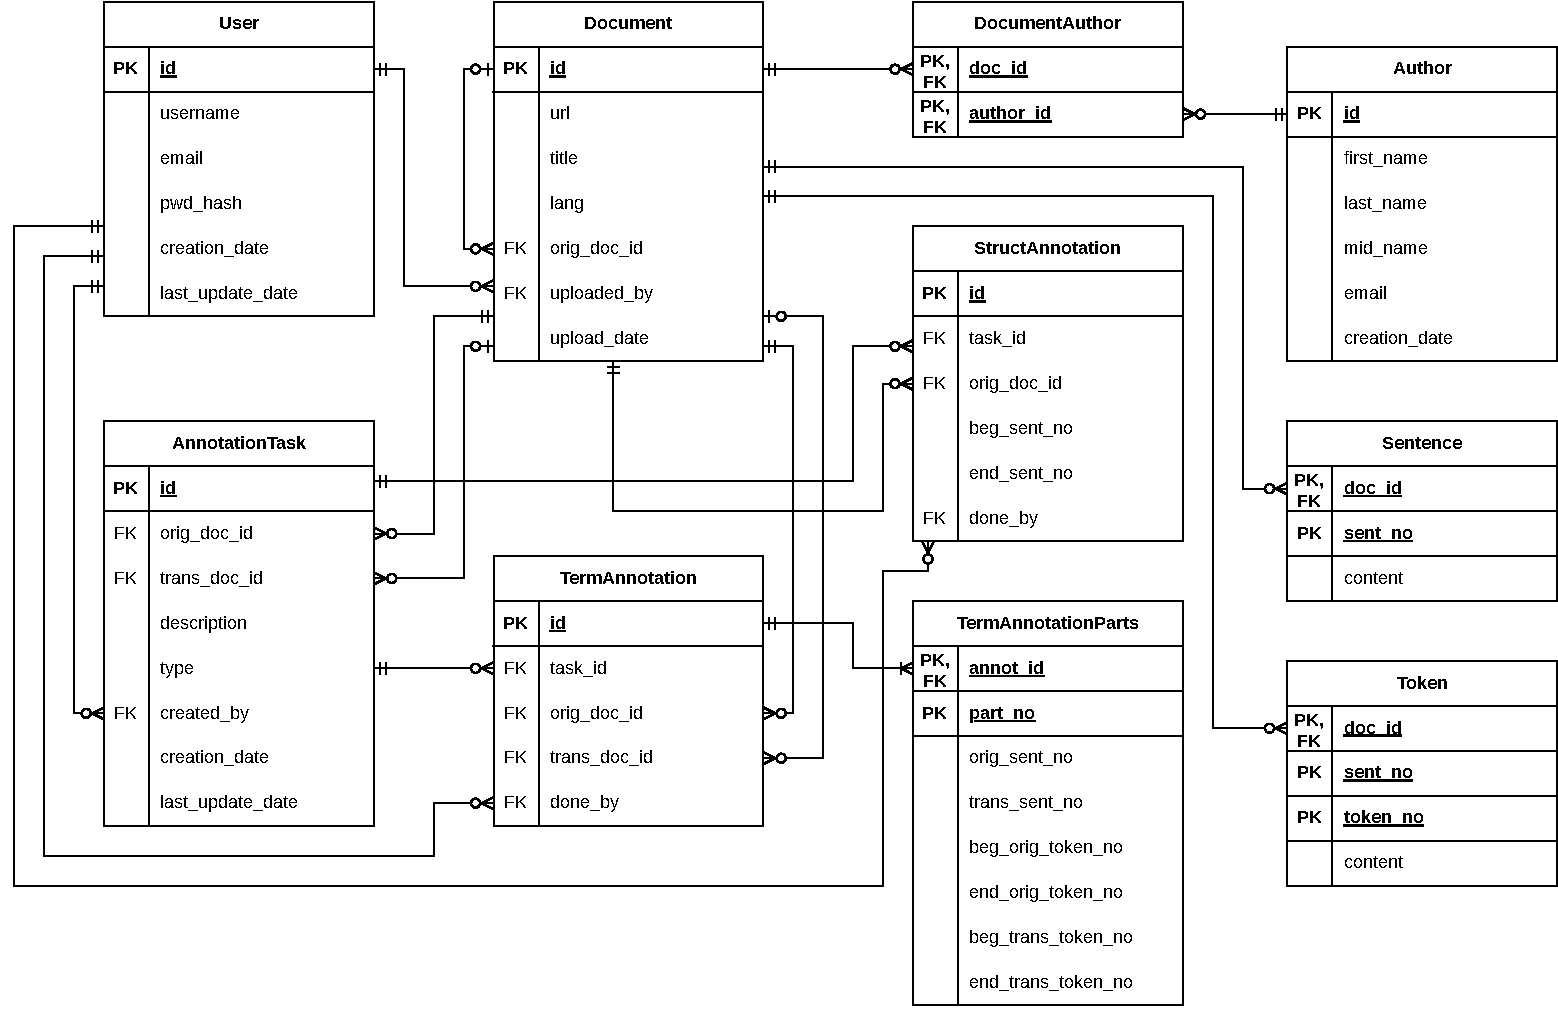
\includegraphics[angle=90, width=0.75\textwidth]{diag/crow-foot-erd.pdf}
	\caption{ER-диаграмма проектируемой базы данных в нотации Мартина}
	\label{fig:erd}
\end{figure}

\subsection{Описание сущностей}

В данном подразделе будут описаны десять сущностей проектируемой базы данных: User, Document, DocumentAuthor, Author, AnnotationTask, StructAnnotation, TermAnnotation, TermAnnotationParts, Sentence, Token.

\subsection{Описание ограничений целостности}

\begin{table}[H]
\centering
\caption{Ограничение целостности User}
\begin{tabular}{|m{4cm}|m{3cm}|m{6cm}|}
\hline
\textbf{Поле} & \textbf{Тип} & \textbf{Ограничение} \\ \hline
id & UUID & первичный ключ \\ \hline
username & строка & уникальный, не пустое значение \\ \hline
email & строка & не пустое значение \\ \hline
pwd\_hash & строка & не пустое значение \\ \hline
creation\_date & временная метка & не пустое значение \\ \hline
last\_update\_date & временная метка & не пустое значение \\ \hline
\end{tabular}
\end{table}

\begin{table}[H]
\centering
\caption{Ограничение целостности Document}
\begin{tabular}{|m{3cm}|m{3cm}|m{6cm}|}
\hline
\textbf{Поле} & \textbf{Тип} & \textbf{Ограничение} \\ \hline
id & UUID & первичный ключ \\ \hline
url & строка & не пустое значение \\ \hline
title & строка & не пустое значение \\ \hline
lang & строка & не пустое значение \\ \hline
orig\_doc\_id & UUID & внешний ключ на поле id таблицы Document \\ \hline
uploaded\_by & UUID & внешний ключ на поле id таблицы User, не пустое значение \\ \hline
upload\_date & временная метка & не пустое значение \\ \hline
\end{tabular}
\end{table}

\begin{table}[H]
\centering
\caption{Ограничение целостности DocumentAuthor}
\begin{tabular}{|m{3cm}|m{3cm}|m{6cm}|}
\hline
\textbf{Поле} & \textbf{Тип} & \textbf{Ограничение} \\ \hline
doc\_id & UUID & первичный ключ, внешний ключ на поле id таблицы Document \\ \hline
author\_id & UUID & первичный ключ, внешний ключ на поле id таблицы Authro \\ \hline
\end{tabular}
\end{table}

\begin{table}[H]
\centering
\caption{Ограничение целостности Author}
\begin{tabular}{|m{3cm}|m{3cm}|m{6cm}|}
\hline
\textbf{Поле} & \textbf{Тип} & \textbf{Ограничение} \\ \hline
id & UUID & первичный ключ \\ \hline
first\_name & строка & --- \\ \hline
last\_name & строка & --- \\ \hline
mid\_name & строка & --- \\ \hline
email & строка & --- \\ \hline
creation\_date & временная метка & не пустое значение \\ \hline
\end{tabular}
\end{table}

\begin{table}[H]
\centering
\caption{Ограничение целостности AnnotationTask}
\begin{tabular}{|m{4cm}|m{3cm}|m{6cm}|}
\hline
\textbf{Поле} & \textbf{Тип} & \textbf{Ограничение} \\ \hline
id & UUID & первичный ключ \\ \hline
orig\_doc\_id & UUID & внешний ключ на поле id таблицы Document, не пустое значение \\ \hline
trans\_doc\_id & UUID & внешний ключ на поле id таблицы Document \\ \hline
description & строка & не пустое значение \\ \hline
type & строка & --- \\ \hline
created\_by & UUID & внешний ключ на поле id таблицы User \\ \hline
creation\_date & временная метка & не пустое значение \\ \hline
last\_update\_date & временная метка & не пустое значение \\ \hline
\end{tabular}
\end{table}

\begin{table}[H]
\centering
\caption{Ограничение целостности StructAnnotation}
\begin{tabular}{|m{3cm}|m{3cm}|m{6cm}|}
\hline
\textbf{Поле} & \textbf{Тип} & \textbf{Ограничение} \\ \hline
id & UUID & первичный ключ \\ \hline
task\_id & UUID & внешний ключ на поле id таблицы AnnotationTask, не пустое значение \\ \hline
orig\_doc\_id & UUID & внешний ключ на поле id таблицы Document, не пустое значение \\ \hline
beg\_sent\_no & целое число & не пустое значение \\ \hline
end\_sent\_no & целое число & не пустое значение \\ \hline
done\_by & UUID & внешний ключ на поле id таблицы User, не пустое значение \\ \hline
\end{tabular}
\end{table}

\begin{table}[H]
\centering
\caption{Ограничение целостности TermAnnotation}
\begin{tabular}{|m{3cm}|m{3cm}|m{6cm}|}
\hline
\textbf{Поле} & \textbf{Тип} & \textbf{Ограничение} \\ \hline
id & UUID & первичный ключ \\ \hline
task\_id & UUID & внешний ключ на поле id таблицы AnnotationTask, не пустое значение \\ \hline
orig\_doc\_id & UUID & внешний ключ на поле id таблицы Document, не пустое значение \\ \hline
trans\_doc\_id & UUID & внешний ключ на поле id таблицы Document \\ \hline
done\_by & UUID & внешний ключ на поле id таблицы User, не пустое значение \\ \hline
\end{tabular}
\end{table}

\begin{table}[H]
\centering
\caption{Ограничение целостности TermAnnotationParts}
\begin{tabular}{|m{5cm}|m{3cm}|m{6cm}|}
\hline
\textbf{Поле} & \textbf{Тип} & \textbf{Ограничение} \\ \hline
annot\_id & UUID & первичный ключ, внешний ключ на поле id таблицы TermAnnotation \\ \hline
part\_no & целое число & первичный ключ \\ \hline
orig\_sent\_no & целое число & не пустое значение \\ \hline
trans\_sent\_no & целое число & не пустое значение \\ \hline
beg\_orig\_token\_no & целое число & не пустое значение \\ \hline
end\_orig\_token\_no & целое число & не пустое значение \\ \hline
beg\_trans\_token\_no & целое число & не пустое значение \\ \hline
end\_trans\_token\_no & целое число & не пустое значение \\ \hline
\end{tabular}
\end{table}

\begin{table}[H]
\centering
\caption{Ограничение целостности Sentence}
\begin{tabular}{|m{3cm}|m{3cm}|m{6cm}|}
\hline
\textbf{Поле} & \textbf{Тип} & \textbf{Ограничение} \\ \hline
doc\_id & UUID & первичный ключ, внешний ключ на поле id таблицы Document \\ \hline
sent\_no & целое число & первичный ключ \\ \hline
content & строка & не пустое значение \\ \hline
\end{tabular}
\end{table}

\begin{table}[H]
\centering
\caption{Ограничение целостности Token}
\begin{tabular}{|m{3cm}|m{3cm}|m{6cm}|}
\hline
\textbf{Поле} & \textbf{Тип} & \textbf{Ограничение} \\ \hline
doc\_id & UUID & первичный ключ, внешний ключ на поле id таблицы Document \\ \hline
sent\_no & целое число & первичный ключ \\ \hline
token\_no & целое число & первичный ключ \\ \hline
content & строка & не пустое значение \\ \hline
\end{tabular}
\end{table}

\subsection{Описание функций, процедур и триггеров}

\subsection{Описание ролевой модели}

\subsection{Вывод}
